
%% bare_jrnl_transmag.tex
%% V1.4a
%% 2014/09/17
%% by Michael Shell
%% see http://www.michaelshell.org/
%% for current contact information.
%%
%% This is a skeleton file demonstrating the use of IEEEtran.cls
%% (requires IEEEtran.cls version 1.8a or later) with an IEEE
%% Transactions on Magnetics journal paper.
%%
%% Support sites:
%% http://www.michaelshell.org/tex/ieeetran/
%% http://www.ctan.org/tex-archive/macros/latex/contrib/IEEEtran/
%% and
%% http://www.ieee.org/

%%*************************************************************************
%% Legal Notice:
%% This code is offered as-is without any warranty either expressed or
%% implied; without even the implied warranty of MERCHANTABILITY or
%% FITNESS FOR A PARTICULAR PURPOSE!
%% User assumes all risk.
%% In no event shall IEEE or any contributor to this code be liable for
%% any damages or losses, including, but not limited to, incidental,
%% consequential, or any other damages, resulting from the use or misuse
%% of any information contained here.
%%
%% All comments are the opinions of their respective authors and are not
%% necessarily endorsed by the IEEE.
%%
%% This work is distributed under the LaTeX Project Public License (LPPL)
%% ( http://www.latex-project.org/ ) version 1.3, and may be freely used,
%% distributed and modified. A copy of the LPPL, version 1.3, is included
%% in the base LaTeX documentation of all distributions of LaTeX released
%% 2003/12/01 or later.
%% Retain all contribution notices and credits.
%% ** Modified files should be clearly indicated as such, including  **
%% ** renaming them and changing author support contact information. **
%%
%% File list of work: IEEEtran.cls, IEEEtran_HOWTO.pdf, bare_adv.tex,
%%                    bare_conf.tex, bare_jrnl.tex, bare_conf_compsoc.tex,
%%                    bare_jrnl_compsoc.tex, bare_jrnl_transmag.tex
%%*************************************************************************


% *** Authors should verify (and, if needed, correct) their LaTeX system  ***
% *** with the testflow diagnostic prior to trusting their LaTeX platform ***
% *** with production work. IEEE's font choices and paper sizes can       ***
% *** trigger bugs that do not appear when using other class files.       ***                          ***
% The testflow support page is at:
% http://www.michaelshell.org/tex/testflow/



\documentclass[journal,transmag]{IEEEtran}
%
% If IEEEtran.cls has not been installed into the LaTeX system files,
% manually specify the path to it like:
% \documentclass[journal]{../sty/IEEEtran}





% Some very useful LaTeX packages include:
% (uncomment the ones you want to load)


% *** MISC UTILITY PACKAGES ***
%
%\usepackage{ifpdf}
% Heiko Oberdiek's ifpdf.sty is very useful if you need conditional
% compilation based on whether the output is pdf or dvi.
% usage:
% \ifpdf
%   % pdf code
% \else
%   % dvi code
% \fi
% The latest version of ifpdf.sty can be obtained from:
% http://www.ctan.org/tex-archive/macros/latex/contrib/oberdiek/
% Also, note that IEEEtran.cls V1.7 and later provides a builtin
% \ifCLASSINFOpdf conditional that works the same way.
% When switching from latex to pdflatex and vice-versa, the compiler may
% have to be run twice to clear warning/error messages.

\usepackage{booktabs}
\usepackage{multirow}
\usepackage{upgreek}


% *** CITATION PACKAGES ***
%
%\usepackage{cite}
% cite.sty was written by Donald Arseneau
% V1.6 and later of IEEEtran pre-defines the format of the cite.sty package
% \cite{} output to follow that of IEEE. Loading the cite package will
% result in citation numbers being automatically sorted and properly
% "compressed/ranged". e.g., [1], [9], [2], [7], [5], [6] without using
% cite.sty will become [1], [2], [5]--[7], [9] using cite.sty. cite.sty's
% \cite will automatically add leading space, if needed. Use cite.sty's
% noadjust option (cite.sty V3.8 and later) if you want to turn this off
% such as if a citation ever needs to be enclosed in parenthesis.
% cite.sty is already installed on most LaTeX systems. Be sure and use
% version 5.0 (2009-03-20) and later if using hyperref.sty.
% The latest version can be obtained at:
% http://www.ctan.org/tex-archive/macros/latex/contrib/cite/
% The documentation is contained in the cite.sty file itself.






% *** GRAPHICS RELATED PACKAGES ***
%
\ifCLASSINFOpdf
% \usepackage[pdftex]{graphicx}
% declare the path(s) where your graphic files are
% \graphicspath{{../pdf/}{../jpeg/}}
% and their extensions so you won't have to specify these with
% every instance of \includegraphics
% \DeclareGraphicsExtensions{.pdf,.jpeg,.png}
\else
% or other class option (dvipsone, dvipdf, if not using dvips). graphicx
% will default to the driver specified in the system graphics.cfg if no
% driver is specified.
% \usepackage[dvips]{graphicx}
% declare the path(s) where your graphic files are
% \graphicspath{{../eps/}}
% and their extensions so you won't have to specify these with
% every instance of \includegraphics
% \DeclareGraphicsExtensions{.eps}
\fi
% graphicx was written by David Carlisle and Sebastian Rahtz. It is
% required if you want graphics, photos, etc. graphicx.sty is already
% installed on most LaTeX systems. The latest version and documentation
% can be obtained at:
% http://www.ctan.org/tex-archive/macros/latex/required/graphics/
% Another good source of documentation is "Using Imported Graphics in
% LaTeX2e" by Keith Reckdahl which can be found at:
% http://www.ctan.org/tex-archive/info/epslatex/
%
% latex, and pdflatex in dvi mode, support graphics in encapsulated
% postscript (.eps) format. pdflatex in pdf mode supports graphics
% in .pdf, .jpeg, .png and .mps (metapost) formats. Users should ensure
% that all non-photo figures use a vector format (.eps, .pdf, .mps) and
% not a bitmapped formats (.jpeg, .png). IEEE frowns on bitmapped formats
% which can result in "jaggedy"/blurry rendering of lines and letters as
% well as large increases in file sizes.
%
% You can find documentation about the pdfTeX application at:
% http://www.tug.org/applications/pdftex




% *** MATH PACKAGES ***
%
%\usepackage[cmex10]{amsmath}
% A popular package from the American Mathematical Society that provides
% many useful and powerful commands for dealing with mathematics. If using
% it, be sure to load this package with the cmex10 option to ensure that
% only type 1 fonts will utilized at all point sizes. Without this option,
% it is possible that some math symbols, particularly those within
% footnotes, will be rendered in bitmap form which will result in a
% document that can not be IEEE Xplore compliant!
%
% Also, note that the amsmath package sets \interdisplaylinepenalty to 10000
% thus preventing page breaks from occurring within multiline equations. Use:
%\interdisplaylinepenalty=2500
% after loading amsmath to restore such page breaks as IEEEtran.cls normally
% does. amsmath.sty is already installed on most LaTeX systems. The latest
% version and documentation can be obtained at:
% http://www.ctan.org/tex-archive/macros/latex/required/amslatex/math/





% *** SPECIALIZED LIST PACKAGES ***
%
%\usepackage{algorithmic}
% algorithmic.sty was written by Peter Williams and Rogerio Brito.
% This package provides an algorithmic environment fo describing algorithms.
% You can use the algorithmic environment in-text or within a figure
% environment to provide for a floating algorithm. Do NOT use the algorithm
% floating environment provided by algorithm.sty (by the same authors) or
% algorithm2e.sty (by Christophe Fiorio) as IEEE does not use dedicated
% algorithm float types and packages that provide these will not provide
% correct IEEE style captions. The latest version and documentation of
% algorithmic.sty can be obtained at:
% http://www.ctan.org/tex-archive/macros/latex/contrib/algorithms/
% There is also a support site at:
% http://algorithms.berlios.de/index.html
% Also of interest may be the (relatively newer and more customizable)
% algorithmicx.sty package by Szasz Janos:
% http://www.ctan.org/tex-archive/macros/latex/contrib/algorithmicx/




% *** ALIGNMENT PACKAGES ***
%
%\usepackage{array}
% Frank Mittelbach's and David Carlisle's array.sty patches and improves
% the standard LaTeX2e array and tabular environments to provide better
% appearance and additional user controls. As the default LaTeX2e table
% generation code is lacking to the point of almost being broken with
% respect to the quality of the end results, all users are strongly
% advised to use an enhanced (at the very least that provided by array.sty)
% set of table tools. array.sty is already installed on most systems. The
% latest version and documentation can be obtained at:
% http://www.ctan.org/tex-archive/macros/latex/required/tools/


% IEEEtran contains the IEEEeqnarray family of commands that can be used to
% generate multiline equations as well as matrices, tables, etc., of high
% quality.




% *** SUBFIGURE PACKAGES ***
%\ifCLASSOPTIONcompsoc
%  \usepackage[caption=false,font=normalsize,labelfont=sf,textfont=sf]{subfig}
%\else
%  \usepackage[caption=false,font=footnotesize]{subfig}
%\fi
% subfig.sty, written by Steven Douglas Cochran, is the modern replacement
% for subfigure.sty, the latter of which is no longer maintained and is
% incompatible with some LaTeX packages including fixltx2e. However,
% subfig.sty requires and automatically loads Axel Sommerfeldt's caption.sty
% which will override IEEEtran.cls' handling of captions and this will result
% in non-IEEE style figure/table captions. To prevent this problem, be sure
% and invoke subfig.sty's "caption=false" package option (available since
% subfig.sty version 1.3, 2005/06/28) as this is will preserve IEEEtran.cls
% handling of captions.
% Note that the Computer Society format requires a larger sans serif font
% than the serif footnote size font used in traditional IEEE formatting
% and thus the need to invoke different subfig.sty package options depending
% on whether compsoc mode has been enabled.
%
% The latest version and documentation of subfig.sty can be obtained at:
% http://www.ctan.org/tex-archive/macros/latex/contrib/subfig/



% *** FLOAT PACKAGES ***
%
%\usepackage{fixltx2e}
% fixltx2e, the successor to the earlier fix2col.sty, was written by
% Frank Mittelbach and David Carlisle. This package corrects a few problems
% in the LaTeX2e kernel, the most notable of which is that in current
% LaTeX2e releases, the ordering of single and double column floats is not
% guaranteed to be preserved. Thus, an unpatched LaTeX2e can allow a
% single column figure to be placed prior to an earlier double column
% figure. The latest version and documentation can be found at:
% http://www.ctan.org/tex-archive/macros/latex/base/


%\usepackage{stfloats}
% stfloats.sty was written by Sigitas Tolusis. This package gives LaTeX2e
% the ability to do double column floats at the bottom of the page as well
% as the top. (e.g., "\begin{figure*}[!b]" is not normally possible in
% LaTeX2e). It also provides a command:
%\fnbelowfloat
% to enable the placement of footnotes below bottom floats (the standard
% LaTeX2e kernel puts them above bottom floats). This is an invasive package
% which rewrites many portions of the LaTeX2e float routines. It may not work
% with other packages that modify the LaTeX2e float routines. The latest
% version and documentation can be obtained at:
% http://www.ctan.org/tex-archive/macros/latex/contrib/sttools/
% Do not use the stfloats baselinefloat ability as IEEE does not allow
% \baselineskip to stretch. Authors submitting work to the IEEE should note
% that IEEE rarely uses double column equations and that authors should try
% to avoid such use. Do not be tempted to use the cuted.sty or midfloat.sty
% packages (also by Sigitas Tolusis) as IEEE does not format its papers in
% such ways.
% Do not attempt to use stfloats with fixltx2e as they are incompatible.
% Instead, use Morten Hogholm'a dblfloatfix which combines the features
% of both fixltx2e and stfloats:
%
% \usepackage{dblfloatfix}
% The latest version can be found at:
% http://www.ctan.org/tex-archive/macros/latex/contrib/dblfloatfix/




%\ifCLASSOPTIONcaptionsoff
%  \usepackage[nomarkers]{endfloat}
% \let\MYoriglatexcaption\caption
% \renewcommand{\caption}[2][\relax]{\MYoriglatexcaption[#2]{#2}}
%\fi
% endfloat.sty was written by James Darrell McCauley, Jeff Goldberg and
% Axel Sommerfeldt. This package may be useful when used in conjunction with
% IEEEtran.cls'  captionsoff option. Some IEEE journals/societies require that
% submissions have lists of figures/tables at the end of the paper and that
% figures/tables without any captions are placed on a page by themselves at
% the end of the document. If needed, the draftcls IEEEtran class option or
% \CLASSINPUTbaselinestretch interface can be used to increase the line
% spacing as well. Be sure and use the nomarkers option of endfloat to
% prevent endfloat from "marking" where the figures would have been placed
% in the text. The two hack lines of code above are a slight modification of
% that suggested by in the endfloat docs (section 8.4.1) to ensure that
% the full captions always appear in the list of figures/tables - even if
% the user used the short optional argument of \caption[]{}.
% IEEE papers do not typically make use of \caption[]'s optional argument,
% so this should not be an issue. A similar trick can be used to disable
% captions of packages such as subfig.sty that lack options to turn off
% the subcaptions:
% For subfig.sty:
% \let\MYorigsubfloat\subfloat
% \renewcommand{\subfloat}[2][\relax]{\MYorigsubfloat[]{#2}}
% However, the above trick will not work if both optional arguments of
% the \subfloat command are used. Furthermore, there needs to be a
% description of each subfigure *somewhere* and endfloat does not add
% subfigure captions to its list of figures. Thus, the best approach is to
% avoid the use of subfigure captions (many IEEE journals avoid them anyway)
% and instead reference/explain all the subfigures within the main caption.
% The latest version of endfloat.sty and its documentation can obtained at:
% http://www.ctan.org/tex-archive/macros/latex/contrib/endfloat/
%
% The IEEEtran \ifCLASSOPTIONcaptionsoff conditional can also be used
% later in the document, say, to conditionally put the References on a
% page by themselves.




% *** PDF, URL AND HYPERLINK PACKAGES ***
%
%\usepackage{url}
% url.sty was written by Donald Arseneau. It provides better support for
% handling and breaking URLs. url.sty is already installed on most LaTeX
% systems. The latest version and documentation can be obtained at:
% http://www.ctan.org/tex-archive/macros/latex/contrib/url/
% Basically, \url{my_url_here}.




% *** Do not adjust lengths that control margins, column widths, etc. ***
% *** Do not use packages that alter fonts (such as pslatex).         ***
% There should be no need to do such things with IEEEtran.cls V1.6 and later.
% (Unless specifically asked to do so by the journal or conference you plan
% to submit to, of course. )


% correct bad hyphenation here
\hyphenation{op-tical net-works semi-conduc-tor}


\usepackage{physics}
\usepackage{mathtools}
\usepackage{mathtools}
\usepackage{listings}

\lstdefinestyle{codeStyleC}{
language=C++,
basicstyle=\ttfamily\small,
keywordstyle=\color{blue}\ttfamily,
stringstyle=\color{red}\ttfamily,
commentstyle=\color{green}\ttfamily,
breaklines=true,
columns=flexible,
gobble=4,
xleftmargin=\leftmargini,
frame=L,
numbers=left,
numberstyle=\tiny,
belowcaptionskip=0.5em,
belowskip=1em,
}

\lstdefinestyle{codeStyleCUDA}{
language=C++,
basicstyle=\ttfamily\small,
keywordstyle=\color{blue}\ttfamily,
keywordstyle=[2]\color{darkgreen},
keywordstyle=[3]\color{red},
stringstyle=\color{red}\ttfamily,
commentstyle=\color{green}\ttfamily,
breaklines=true,
columns=flexible,
gobble=4,
xleftmargin=\leftmargini,
frame=L,
numbers=left,
numberstyle=\tiny,
keywords=[2]{__global__,__host__,__device__,__synchThreads()},
keywords=[3]{atomicAdd},
belowcaptionskip=1em,
belowskip=1em,
}

\lstdefinestyle{codeStyleFORTRAN}{
language=FORTRAN,
basicstyle=\ttfamily\small,
keywordstyle=\color{blue}\ttfamily,
keywordstyle=[2]\color{darkgreen},
stringstyle=\color{red}\ttfamily,
commentstyle=\color{green}\ttfamily,
breaklines=true,
columns=flexible,
gobble=4,
xleftmargin=\leftmargini,
frame=L,
numbers=left,
numberstyle=\tiny,
keywords=[2]{__global__,__host__,__device__,__synchThreads()},
belowcaptionskip=2em,
belowskip=5em,
}

\begin{document}

%
% paper title
% Titles are generally capitalized except for words such as a, an, and, as,
% at, but, by, for, in, nor, of, on, or, the, to and up, which are usually
% not capitalized unless they are the first or last word of the title.
% Linebreaks \\ can be used within to get better formatting as desired.
% Do not put math or special symbols in the title.
\title{Multi-Agent System with Multiple Group Modelling for Bird Flocking
on GPU}



% author names and affiliations
% transmag papers use the long conference author name format.

% 		\author{\IEEEauthorblockN{Rahmat Hidayat\IEEEauthorrefmark{1,2},
% 		Davide Spataro\IEEEauthorrefmark{2},
% 		William Spataro\IEEEauthorrefmark{2},
% 		Donato D'Ambrosio\IEEEauthorrefmark{2}}
% 		
% 		\IEEEauthorblockA{\IEEEauthorrefmark{1}University Of Calabria,
% 		Department of Mathematics and Computer Science, Italy}
% 		\IEEEauthorblockA{\IEEEauthorrefmark{2}IT Division BPJS Kesehatan, Indonesia}
% 		}

%\thanks{Manuscript received December 1, 2012; revised September 17, 2014.
%Corresponding author: M. Shell (email:
% http://www.michaelshell.org/contact.html).}}



% The paper headers
%\markboth{Journal of \LaTeX\ Class Files,~Vol.~13, No.~9, September~2014}%
%{Shell \MakeLowercase{\textit{et al.}}: Bare Demo of IEEEtran.cls for Journals}
% The only time the second header will appear is for the odd numbered pages
% after the title page when using the twoside option.
%
% *** Note that you probably will NOT want to include the author's ***
% *** name in the headers of peer review papers.                   ***
% You can use \ifCLASSOPTIONpeerreview for conditional compilation here if
% you desire.




% If you want to put a publisher's ID mark on the page you can do it like
% this:
%\IEEEpubid{0000--0000/00\$00.00~\copyright~2014 IEEE}
% Remember, if you use this you must call \IEEEpubidadjcol in the second
% column for its text to clear the IEEEpubid mark.



% use for special paper notices
%\IEEEspecialpapernotice{(Invited Paper)}


% for Transactions on Magnetics papers, we must declare the abstract and
% index terms PRIOR to the title within the \IEEEtitleabstractindextext
% IEEEtran command as these need to go into the title area created by
% \maketitle.
% As a general rule, do not put math, special symbols or citations
% in the abstract or keywords.
\IEEEtitleabstractindextext{%
\begin{abstract}
Birds flocking is an interesting natural phenomenon to study as proven by
numerous papers in this field. In this paper, we present a massive birds
flocking simulation using the GPGPU CUDA framework. This technology has been
widely adopted in computational science fields and dramatically increase
computation performances. Using the autonomous agent approach with multi-agents
and multiple groups for birds flocking modeling, we present both aggregate
motion of a large number of birds in virtual environment and other species or
predators avoidance in the plane as well. From  these experiments we gained
significant performance improvements in the terms of speedup. In
conclusion, the work shows that the use of  the CUDA technology can be effective
to cut computational costs also in multi agent modeling.
\end{abstract}

% Note that keywords are not normally used for peerreview papers.
\begin{IEEEkeywords}
GPGPU, CUDA, flocking, modelling.
\end{IEEEkeywords}}



% make the title area
\maketitle


% To allow for easy dual compilation without having to reenter the
% abstract/keywords data, the \IEEEtitleabstractindextext text will
% not be used in maketitle, but will appear (i.e., to be "transported")
% here as \IEEEdisplaynontitleabstractindextext when the compsoc
% or transmag modes are not selected <OR> if conference mode is selected
% - because all conference papers position the abstract like regular
% papers do.
\IEEEdisplaynontitleabstractindextext
% \IEEEdisplaynontitleabstractindextext has no effect when using
% compsoc or transmag under a non-conference mode.







% For peer review papers, you can put extra information on the cover
% page as needed:
% \ifCLASSOPTIONpeerreview
% \begin{center} \bfseries EDICS Category: 3-BBND \end{center}
% \fi
%
% For peerreview papers, this IEEEtran command inserts a page break and
% creates the second title. It will be ignored for other modes.
\IEEEpeerreviewmaketitle



\section{Introduction}
% The very first letter is a 2 line initial drop letter followed
% by the rest of the first word in caps.
%
% form to use if the first word consists of a single letter:
% \IEEEPARstart{A}{demo} file is ....
%
% form to use if you need the single drop letter followed by
% normal text (unknown if ever used by IEEE):
% \IEEEPARstart{A}{}demo file is ....
%
% Some journals put the first two words in caps:
% \IEEEPARstart{T}{his demo} file is ....
%
% Here we have the typical use of a "T" for an initial drop letter
% and "HIS" in caps to complete the first word.
\IEEEPARstart{B}{ird} flocking is a natural phenomenon that is very interesting to be
studied. It is proven by numerous papers published in this field that
are related with both biological and computer science. Several years
ago, people were wondering about this phenomenon. Why birds flocking together?
How they communicate each other and form fascinate formation in the space? Many models have been proposed regarding
this phenomenon. It is believed that the most successful and famous
is boid (a contraction from bird-oid) proposed by Craig W. Reynolds
(1987). 


% An example of a floating figure using the graphicx package.
% Note that \label must occur AFTER (or within) \caption.
% For figures, \caption should occur after the \includegraphics.
% Note that IEEEtran v1.7 and later has special internal code that
% is designed to preserve the operation of \label within \caption
% even when the captionsoff option is in effect. However, because
% of issues like this, it may be the safest practice to put all your
% \label just after \caption rather than within \caption{}.
%
% Reminder: the "draftcls" or "draftclsnofoot", not "draft", class
% option should be used if it is desired that the figures are to be
% displayed while in draft mode.
%
%\begin{figure}[!t]
%\centering
%\includegraphics[width=2.5in]{myfigure}
% where an .eps filename suffix will be assumed under latex,
% and a .pdf suffix will be assumed for pdflatex; or what has been declared
% via \DeclareGraphicsExtensions.
%\caption{Simulation results for the network.}
%\label{fig_sim}
%\end{figure}

% Note that IEEE typically puts floats only at the top, even when this
% results in a large percentage of a column being occupied by floats.


% An example of a double column floating figure using two subfigures.
% (The subfig.sty package must be loaded for this to work.)
% The subfigure \label commands are set within each subfloat command,
% and the \label for the overall figure must come after \caption.
% \hfil is used as a separator to get equal spacing.
% Watch out that the combined width of all the subfigures on a
% line do not exceed the text width or a line break will occur.
%
%\begin{figure*}[!t]
%\centering
%\subfloat[Case I]{\includegraphics[width=2.5in]{box}%
%\label{fig_first_case}}
%\hfil
%\subfloat[Case II]{\includegraphics[width=2.5in]{box}%
%\label{fig_second_case}}
%\caption{Simulation results for the network.}
%\label{fig_sim}
%\end{figure*}
%
% Note that often IEEE papers with subfigures do not employ subfigure
% captions (using the optional argument to \subfloat[]), but instead will
% reference/describe all of them (a), (b), etc., within the main caption.
% Be aware that for subfig.sty to generate the (a), (b), etc., subfigure
% labels, the optional argument to \subfloat must be present. If a
% subcaption is not desired, just leave its contents blank,
% e.g., \subfloat[].


% An example of a floating table. Note that, for IEEE style tables, the
% \caption command should come BEFORE the table and, given that table
% captions serve much like titles, are usually capitalized except for words
% such as a, an, and, as, at, but, by, for, in, nor, of, on, or, the, to
% and up, which are usually not capitalized unless they are the first or
% last word of the caption. Table text will default to \footnotesize as
% IEEE normally uses this smaller font for tables.
% The \label must come after \caption as always.
%
%\begin{table}[!t]
%% increase table row spacing, adjust to taste
%\renewcommand{\arraystretch}{1.3}
% if using array.sty, it might be a good idea to tweak the value of
% \extrarowheight as needed to properly center the text within the cells
%\caption{An Example of a Table}
%\label{table_example}
%\centering
%% Some packages, such as MDW tools, offer better commands for making tables
%% than the plain LaTeX2e tabular which is used here.
%\begin{tabular}{|c||c|}
%\hline
%One & Two\\
%\hline
%Three & Four\\
%\hline
%\end{tabular}
%\end{table}


% Note that the IEEE does not put floats in the very first column
% - or typically anywhere on the first page for that matter. Also,
% in-text middle ("here") positioning is typically not used, but it
% is allowed and encouraged for Computer Society conferences (but
% not Computer Society journals). Most IEEE journals/conferences use
% top floats exclusively.
% Note that, LaTeX2e, unlike IEEE journals/conferences, places
% footnotes above bottom floats. This can be corrected via the
% \fnbelowfloat command of the stfloats package.


\section{Flocking Model}\label{sec:model}
\IEEEPARstart{T}{his} work is  based on flocking behavior that was proposed by
Craig W. Reynolds in 1987 and extends it by adding the support to coexistence
and interaction between different species and predator avoidance.
Intuitively the model is regulated by the following rules:
\begin{description}
\item[\textsc{Cohesion}] \hfill\\
	birds always tend to go to the center of mass, i.e.
the center position of its neighbors
\item[\textsc{Separation}] \hfill\\
	birds always keep certain distance between itself to its neighbor
\item[\textsc{Alignment}] \hfill\\
	bird always tend to match its velocity with its nearby flockmates
\end{description}

Bird flight at step $i$ is decribed by its position
$\vb{p^i_b}=\expval{p^i_x,p^i_y,p^i_z}$ and velocity
$\vb{v^i_b}=\expval{p^i_x,p^i_y,p^i_z}$. 
At high level, the evolution of the bird's  velocity over time is regulated by
the following: $\vb{v^{i+1}_b}=\mu_c \vec{v}^i_c + \mu_s \vec{v}^i_s +\mu_a
\vec{v}^i_a$ where:

\begin{itemize}
  \item $\mu_c$,$\mu_s$,$\mu_a$ are the cohesion, separation and alignment
  coefficient, respectively
  \item $\vec{v}^i_c$, the cohesion velocity, has direction parallel to the line
  that pass throug $\vb{p^i_b}$ and the averge of the positions of its neighbors
  \item $\vec{v}^i_s$, the separation velocity, keep the bird at a minimum
  safety distance from its flockmates
  \item  $\vec{v}^i_c$, the align velocity, synchronize boids heading
\end{itemize}


\subsection{Simulation Parameters}
The model takes a number of sets of parameters, for describing the environment
and specifying the bird species, respectively.
 
 \subsubsection{Environment Parameter}
 The environment is described by means of its width, length, height and by the
 time step parameter i.e. the duration in seconds of a single computational
 step. 
 \begin{table}[h!]
	\centering
	\begin{tabular}{l l l l}
	\toprule
	\tabhead{Name} & \tabhead{Symbol} & \tabhead{Dimension} & \tabhead{Description}\\
	\midrule
	Length & \(W_x\) & \(\dimens{L}\) & Length of the environment \\
	Height & \(W_y\) & \(\dimens{L}\) & Height of the environment \\
	Width & \(W_z\) & \(\dimens{L}\) & Width of the environment \\
	Time Step & \(t\) & \(\dimens{T}\) & computational step duration \\
	\bottomrule
	\end{tabular}
	\caption[List of Environment Parameters]{List of Environment Parameters of Birds Flocking}
	\label{tab:EnvironmentParameters}
\end{table}


\(W_x\), \(W_y\), and \(W_z\) are the dimension of the environment that represent 1 pixel as 1 meter. \(t\) is computational duration where 1 time step equivalent to 1 processing time.

\subsubsection{Species Parameters}
Each birds come with a set of parameters that describe physical quantities that are involved in the flight and flock dynamics. The parameters are:

\begin{table*}
\centering
	\begin{tabular}{|l | l| l| l|}
	\hline
	\tabhead{Name} & \tabhead{Symbol} & \tabhead{Dimension} & \tabhead{Description}\\
	\hline
	Size & s\) & \(\dimens{L}\) & Size of the bird \\
	Peak Velocity & \(v_p\)  & \( \dimens{L} \dimens{T^{-1}}\)  & The maximum velocity\\
	Thrust 	& \(a\) & \( \dimens{L} \dimens{T^{-2}}\)  & The maximum acceleration\\
	Horizontal Range of View & \(s_h\) & \(-\) & Maximum horizontal range of view\\ 
	Vertical Range of View & \(s_v\) 	& \(-\) & Maximum vertical range of view\\
	Sight Distance & \(d_s\) & \( \dimens{L}\) & Maximum sight distance\\
	Minimum Distance & \(d_{min}\) & \( \dimens{L}\)  & The minimum distance between two birds to avoid collision\\
	Alignment Radius & \(d_a\) & \( \dimens{L}\)  & The maximum distance bird consider to align\\
	Other Species Avoidance Radius & \(r_s\) & \( \dimens{L}\) & The minimum distance bird avoid other species\\
	Predator Avoidance Radius & \(r_p\) & \( \dimens{L}\) & The minimum distance bird avoid predator\\
	Maximum Turn & \(\theta_{max}\) & \( rad \dimens{s^{-1}} \) & Maximum turn for each time step\\
	Wander Distance & \(w_d\) & \( rad \dimens{s^{-1}} \) & The maximum wandering distance\\
	Wander Radius & \(w_r\)	& \( rad \dimens{s^{-1}} \) & The maximum radius wandering from the target\\
	\hline
	\end{tabular}
	\hfill \\
	\caption[List of Bird Parameters]{List of Bird Parameters with values considered for the simulation}
	\label{tab:BirdParameters}
\end{table*}

The  bird's wingspan \(s\) and is used as an approximation of the volume
it occupies. \(v_p\) is the maximum velocity it can travel and \(a\) represents bird's maximum acceleration.
Each bird has a limited sight of view that is described by its maximum
horizontal, \(s_h\), and vertical, \(s_v\) field of view (see images
\ref{fig:hfow} \ref{fig:vfow} and by \(d_s\) that is the maximum sight distance
of bird i.e. the maximum distance at wich the bird can obsers objects.
Vertical,Horizontal field of view and maximum sight distance defines the viewing 
frustum.


\begin{figure}[h!]
\centering
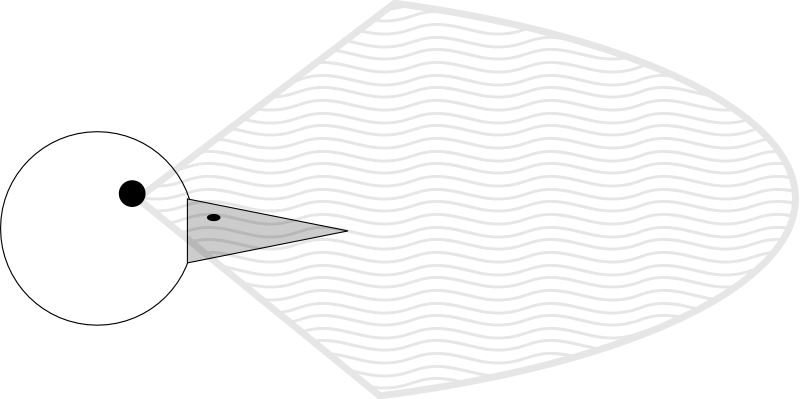
\includegraphics[scale=0.38]{./images/verticalFow.png}
\caption[Horizontal field of view]{Vertical field of view}
\label{fig:hfow}
\end{figure}


\begin{figure}[h!]
\centering
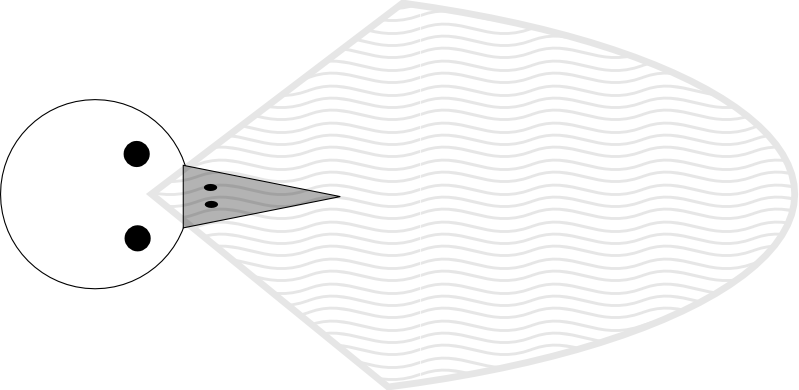
\includegraphics[scale=0.38]{./images/hFow.png}
\caption[Simulation of 605 birds on sequential application]{Horizontal field of
view}
\label{fig:vfow}
\end{figure}

% \begin{figure}
% \centering
% 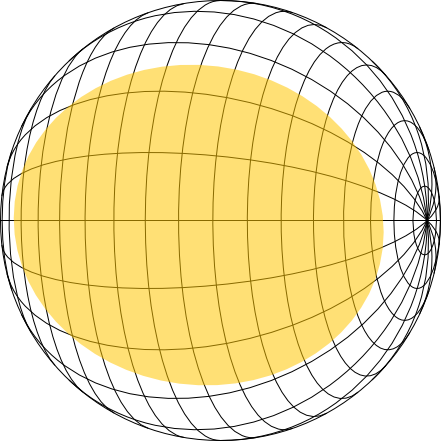
\includegraphics[scale=0.38]{./images/fow.png}
% \caption[Simulation of 605 birds on sequential application]{Vertical field of
% view}
% \label{fig:vfow}
% \end{figure}

\pagebreak

\subsection{Neighborhood}
Each bird has a limited visual capacity described by its field of view. This
implies that it can only perceive as neghbors those birds that are within its
FOV. In order a bird  $n$ to be withing the  observer's neighborhood $o$ it must
fall withing its viewing frustum. Let $\vb{p_r}=\expval{x',y',z'} = \vec{p}_{n}
- \vec{p}_{o}$, $\vb{p_o}=\expval{x,y,z}$ then $\alpha = arctan
\left[\frac{y}{x}\right]$, $\beta = arctan \left[\frac{z}{\sqrt{x^2 +
y^2}}\right]$, $\alpha' = arctan\left[\frac{y'}{x'}\right]$, $\beta = arctan
\left[\frac{z'}{\sqrt{x'^2 + y'^2}}\right]$. Then a bird $n$ is in the
neighborhoof of $o$ if the followings hold:
\begin{align}
&\delta_p = |\vec{p}_{n} - \vec{p}_{o}|,\;\; \delta_p \leq d_s\\
&\Delta_\alpha = \left|\frac{\alpha - \alpha'}{2}\right|,\;\; 0 \leq \Delta_\alpha \leq s_h\\
&\Delta_\beta = \left|\frac{\beta - \beta'}{2}\right|,\;\; 0 \leq \Delta_\beta \leq s_v
\end{align}



\subsection{Cohesion}
Cohesion is a behavior that steer a bird goes to the center of mass, by means average position of its neighbors. A bird compute all of its neighbors, then determine the average position. To go to the center of mass using seek behavior. In formal terms, the center of mass is given by:

\begin{align}
\vec{C}_i = \frac{1}{m}\sum_{n=1}^m{\vec{p}_n f_c}
\end{align}

where:

\begin{enumerate}
\item \(\vec{C}_i\) is the center of mass or average position of neighbors of bird \emph{i}-th
\item \(m\) is the number of neighbors (same species)
\item \(\vec{p}_n\) is the position of \emph{n}-th neighbor
\item \(f_c\) is the weight function, suppose \(d_{i,j}\) is the distance between bird \emph{i} to its neighbor \emph{j}, the weight function \(f_c\) given by:

\begin{equation*}
	f_c = \begin{cases}
	0 &\text{, if $ d_{i,j} > d_s$}\\
	\frac{d_{i,j}}{d_s} &\text{, otherwise}
	\end{cases}
\end{equation*}

\end{enumerate}

Suppose \(\vec{p}_i\) is the position of bird \emph{i}-th, \(\vec{v}_c\) is the cohesion vector, and \(a\) and \(t\) are respectively acceleration and time step, in which drive the observer to the center of mass. To compute the cohesion force given by:

\begin{align}
\vec{v}_d = \frac{\vec{C}_i - \vec{p}_i}{| \vec{C}_i - \vec{p}_i |} + at, \;\;0 < |\vec{v}_d| \leq v_p
\end{align}

\subsection{Separation}
During flying, the birds always try to keep certain distance between itself and its neighbors. This behavior called \emph{separation}. In general, this behavior similar with flee. The difference is in flee the bird consider only to one object, but in separation the bird consider to its neighbor position. To compute the separation force given by:

\begin{align}
\vec{S}_i = \left[\sum_{n=1}^m{\frac{\vec{p}_i - \vec{p}_j}{|\vec{p}_i - \vec{p}_j|^2}} \;f_s\right] + at, \;\;0 < |\vec{S}_i| \leq v_p
\end{align}

where:

\begin{enumerate}
\item \(\vec{S}_i\) is the separation force of bird \emph{i}-th. 
\item \(m\) is the number of neighbors (same species)
\item \(\vec{p}_i\) is the vector position of bird \emph{i}-th.
\item \(\vec{p}_j\) is the vector position of neighbor \emph{j}-th.
\item \(f_s\) is the weight function, suppose \(d_{i,j}\) is the distance between bird \emph{i} to its neighbor \emph{j}, the weight function \(f_s\) given by:

\begin{equation*}
	f_s = \begin{cases}
	0 &\text{, if $ d_{i,j} > d_min$}\\
	1 - \frac{d_{i,j}}{d_{min}} &\text{, otherwise}
	\end{cases}
\end{equation*}
\end{enumerate}

\subsection{Alignment}
In flocking behavior, bird try to match its velocity (speed and heading) with nearby flockmates. In real life bird does not consider to all its neighbors, but only a small number of them limited by certain distance. For example, dove only interact with about seven neighbors \cite{phys.org}. In fact, alignment behavior is just cumulative sum of neighbor's velocity. In formal terms, it given by:

\begin{align}
\vec{A}_i = \left[\sum_{n=1}^m{\vec{v_n}}\;f_a\right] + at, \;\;0 < |\vec{A}_i| \leq v_p
\end{align}

where:

\begin{enumerate}
\item \(\vec{A}_i\) is the alignment force of bird \emph{i}-th. 
\item \(m\) is the number of birds which are considered to align.
\item \(\vec{v}_n\) is the velocity of neighbor \emph{n}-th.
\item \(f_a\) is the weight function, suppose \(d_{i,j}\) is the distance between bird \emph{i} to its neighbor \emph{j}, the weight function \(f_a\) given by:

\begin{equation*}
	f_a = \begin{cases}
	0 &\text{, if $ d_{i,j} > d_a$}\\
	1- \frac{d_{i,j}}{d_a} &\text{, otherwise}
	\end{cases}
\end{equation*}
\end{enumerate}

\subsection{Collision Avoidance}

As mention above (see \ref{tab:BirdParameters}), this thesis modeled birds flocking in multi-agent with multiple group. In order to model in which a bird avoid collision and separate with other species and evade from predator which is try to chase it, it is necessary distinguish those two behaviors. 

\begin{enumerate}[-]
\item \textbf{Other species avoidance}

Other species avoidance behavior more less like separation, the difference is: in this behavior the bird only consider with the neighbors from different species. The bird enumerates its neighbor from difference species, then flee from them. With this behavior, bird will flee from other group, by means other species, and flock together with the same species. In formal terms, it is given by:

\begin{align}
\vec{\uptau}_i = \left[\sum_{n=1}^m{\frac{\vec{p}_i - \vec{p}_j}{|\vec{p}_i - \vec{p}_j|^2}} \;f_{sa}\right] + at, \;\;0 < |\vec{\uptau}_i| \leq v_p
\end{align}

where:

\begin{enumerate}
\item \(\vec{\uptau}_i\) is the avoidance force of bird \emph{i}-th. 
\item \(m\) is the number of neighbors (other species)
\item \(\vec{p}_i\) is the vector position of bird \emph{i}-th.
\item \(\vec{p}_j\) is the vector position of other species \emph{j}-th.
\item \(f_{sa}\) is the weight function, suppose \(d_{i,j}\) is the distance between bird \emph{i} to other species \emph{j}, the weight function \(f_{sa}\) given by:

\begin{equation*}
	f_{sa} = \begin{cases}
	0 &\text{, if $ d_{i,j} > r_s$}\\
	1 - \frac{d_{i,j}}{r_s} &\text{, otherwise}
	\end{cases}
\end{equation*}
\end{enumerate}

\item \textbf{Predator avoidance}

This behavior is evasion in group flocking. Instead only flee from other object (in this case is predator), a bird also consider to the velocity of that object. In other words, a bird checks if whether predator near itself, then if any it compute predator's position and its velocity then evades from the predator. In formal terms, it given by:

\begin{align}
\vec{\Gamma}_i = \left[\sum_{n=1}^m{\frac{\vec{p}_i - (\vec{p}_j+\vec{v}_j)}{|\vec{p}_i - (\vec{p}_j+\vec{v}_j)|^2}} \;f_{pa}\right] + at, \;\;0 < |\vec{\Gamma}_i| \leq v_p
\end{align}

where:

\begin{enumerate}
\item \(\vec{\Gamma}_i\) is the avoidance force of bird \emph{i}-th.
\item \(m\) is the number of predators 
\item \(\vec{p}_i\) is the vector position of bird \emph{i}-th.
\item \(\vec{p}_j\) is the vector position of predator \emph{j}-th.
\item \(\vec{v}_j\) is the vector velocity of predator \emph{j}-th.
\item \(f_{pa}\) is the weight function, suppose \(d_{i,j}\) is the distance between bird \emph{i} to predator \emph{j}, the weight function \(f_{pa}\) given by:

\begin{equation*}
	f_{pa} = \begin{cases}
	0 &\text{, if $ d_{i,j} > r_p$}\\
	1 - \frac{d_{i,j}}{r_p} &\text{, otherwise}
	\end{cases}
\end{equation*}
\end{enumerate}
\end{enumerate}

\subsection{Wandering}
Sometime a bird fly far from its neighbor or can not find its neighbors. In order to find its neighbor, a bird fly randomly in the space, this behavior called wandering. Suppose \(rand()\) is a function to generate random vector and \(\mathbb{N}\) is its neighbors, wandering force given by:

\begin{align}
&\vec{s} = rand(), \;\;\vec{s} \leq \vec{W}\\
&\vec{\omega}_i = \begin{cases}
		0 &\text{, if $ \mathbb{N} \neq \emptyset$}\\
		\frac{\vec{s}}{|\vec{s}|}\;w_r+w_d,\; 0 < |\vec{\omega}_i| \leq v_p &\text{, otherwise}
	\end{cases}
\end{align}


\subsubsection{Desired Velocity}

Desired velocity is summation of those forces. Suppose \(\mu_{av}\) is coefficient avoidance, since we also consider to other species and predator avoidance and wandering, desired velocity \(\vec{v_d}\) given by:

\[
\vec{v}_d = \mu_c \vec{v}_c + \mu_s\vec{v}_s + \mu_a\vec{v}_a + \mu_{av} \left( \vec{\uptau}_i + \vec{\Gamma}_i \right) + \vec{\omega}_i, \;\;0 < |\vec{v}_d| \leq v_p\\
\]

Since a bird can not changes its direction radically, it is limited by maximum turn, in which this behavior given by:

\begin{align}
\vec{v'}_d = \frac{|\vec{v}_d|}{|\vec{v}_{pr}|}\left( \left[1 - \theta_t\right]\vec{v}_{pr} + \theta_t\vec{v}_d\right), \;\theta_t \in \left[0..1\right]
\end{align}

where:

\begin{enumerate}
\item \(\vec{v'}_d\) is desired velocity after adjustment with next velocity angle
\item \(\vec{v}_{pr}\) is previous velocity of the bird
\item \(\vec{v}_d\) is desired velocity before adjustment
\item \(\theta_t\) is adjustment factor, suppose \(\theta\) is angle between previous velocity and desired velocity, its calculation is given by:

\begin{equation*}
\theta_t = \begin{cases}
0 &\text{, if $ \theta = 0$}\\
\frac{\theta_{max}}{\theta}&\text{, otherwise}
\end{cases}
\end{equation*}
\end{enumerate}


\section{Parallel implementation}
In this work we adopt GPUs to accelerate flocking simulation using the the model
presented in section \ref{sec:model} in an environment with a number of agents up to $5 \times10^6$.
Seeking the APOD parallelizing methodology we produced two parallel version.
The two version share the high-level implementation structure that consists
in(the well-known host-managed accelerated program structure): 
\begin{itemize}
	\item Initialization of data structures on CPU
	\item Memory copies from CPU to GPU
	\item Kernels execution on GPU
	\item Copying the result back from GPU to CPU
\end{itemize}
The parallelization strategy is designed in purpose to avoid as much
as possible the very undesirable copies data back and forth from CPU to GPU.
A 3D visualization tool comes with the simulation system and permits real time
rendering of the flocking model.

\subsection{Na\"{i}ve version}
In this version each agent is mapped to a CUDA thread. All data
resides in global memory and shared memory remains unutilized. Altough its simplicity this
version already yeld to a speedup of $\approx20 \times$. 


\subsection{If-divergence mitigation version}
Thread divergence is a well known issue, that disallow full parallelism at warp
level. The most common code construct that can cause thread divergence is
branching for conditionals in an if-then-else statement. If some threads in a single warp evaluate to 'true' and others to
'false', then the 'true' and 'false' threads will branch to different
instructions. Some threads will want proceed to the 'then' instruction, while
others the 'else'.

Intuitively, we would think statements in then and else should be executed in
parallel. However, because of the requirement that threads in a warp cannot
diverge, this cannot happen. The CUDA platform has a workaround that fixes the
problem, but has negative performance consequences.

When executing the if-then-else statement, the CUDA platform will instruct the
warp to execute the then part first, and then proceed to the else part. While
executing the then part, all threads that evaluated to false (e.g. the else
threads) are effectively deactivated. When execution proceeds to the else
condition, the situation is reversed. As you can see, the then and else parts
are not executed in parallel, but in serial. This serialization can result in a
significant performance loss.
In order to mitigate this problem a serie of workaraound have been implemented,
and more specifically, a number of $if$ construct have been substituted with
equivalent arithmetical operation that are performed by all thread in the same
warp, that not change the original semantic of the code. 

If divergence mitigation will reduce execution time as well, since CUDA
parallelization of each thread execute the same code. It means that,
there is an idle time while a thread waiting other threads finished their
task. 
\section{Experimental results}
In order to ensure the correctness of the parallelization the output of each
parallel version were matched against the corrensponding serial output. 



\subsection{Hardware}
Three  devices were adopted for testing different CUDA version of the
model, the high-end GTX 980, Tesla K40 and a GT 635M,a low-end mobile chip(see
table \ref{tab:adoptedHW} for further details).

 \begin{table}
	\centering
	\begin{tabular}{|l |l |l| l|l|}
	\hline
	\ {Name} & \tabhead{Compute Capability} & \tabhead{RAM} &
	\tabhead{SM-Clock} & \tabhead{\# cores}\\
	\hline
	GT 653M & \(2.1\) & \(1024\)MB  & $675$ MHz  & 635\\
	GTX 980& \(5.5\) & \(4096\)MB  & $1216$ MHz & 2048 \\
	TESLA K40& \(5.2\) & \(12288\)MB  & $875$ MHz & 2880 \\
	\hline
	\end{tabular}
	\caption{Hardware utilized for experiments}
	\label{tab:adoptedHW}
\end{table}

a low end mobile chip and a high-end GPU GT 635M, compute capability 2.1 and GTX 980

\subsection{Timings}
See table \ref{tab:naive} and \ref{tab:ifdiv}.

\begin{table}[h!]
	\centering
	\begin{tabular}{|l |l |l| l| l|}
	\hline
	\tabhead {\# birds} & \tabhead{Sequential} & \tabhead{GT
	635M} & \tabhead{GTX 980} & \tabhead{TESLA K40}
	\\
	\hline
	
	1024  & \(263.9\) & $29.1$ & $10.5$ & -\\
	5120  & \(4913.0\) & $574.4$ & $51.7$ & - \\
	10240 &  $19074.5$ & 2241.6 & 109.0 & - \\
	15360  & \(43332.3\) & $5004.7$ & $235.2$ & - \\
	20480  & 86065.7 & 8868.9 & $312.5$ & - \\
	40960  & 452423.1 & - & $1023.8$ & - \\
	81920  & 1966134.9 & - & $3663.5$ & - \\
	163840  & 8003173.0 & - & $14877.4$ & - \\
	327680  & 35815012.0 & - & $58003.0$ & - \\
	\hline
	\end{tabular}
	\caption{Timing (in seconds) for the Parallel CUDA Na\"ive implementation}
	\label{tab:naive}
\end{table}

\begin{table}[h!]
	\centering
	\begin{tabular}{|l |l |l| l| l|}
	\hline
	\tabhead {\# birds} & \tabhead{Sequential} & \tabhead{GT
	635M} & \tabhead{GTX 980} & \tabhead{TESLA K40}
	\\
	\hline
	
	1024  & \(263.9\) & $19.9$ & $7.9$ & - \\
	5120  & \(4913.0\) & $366.3$ & $34.6$ & - \\
	10240 &  $19074.5$ & 1398.7 & 96.5 & - \\
	15360  & \(43332.3\) & $3110.0$ & $154.9$ & - \\
	20480  & 86065.7 & 5522.0 & $280.8$ & - \\
	40960  & 452423.1 & - & $825.4$ & - \\
	81920  & 1966134.9 & - & $3307.2$ & - \\
	163840  & 8003173.0 & - & $13565.9$ & - \\
	327680  & 35815012.0 & - & $54113.4$ & - \\
	\hline
	\end{tabular}
	\caption{Timing (in seconds) for the Parallel CUDA If-Divergence implementation}
	\label{tab:ifdiv}
\end{table}


\section{Conclusion}
In conclusion, the work shows that the use of the CUDA technology can be effective to cut computational costs also in multi agent
modeling.

\subsection{Future development}
Although Reynold’s model is very good, but we also need future im-
provement in order to make simulation as well as in the real world.
Adding some parameters are needed in order to mimic how bird fly.

\(v_s\) is stall velocity, in which a minimum bird's velocity. If a bird fly with velocity lower than its stall velocity, the bird will stall. \(v_c\) is the normal velocity of bird. Bird always tends to fly with \(v_c\) when it fly in group. Since a bird can not fly in vertical way, it is necessary to add a parameter to represent this limitation. \(\Theta_{max}\) is the maximum angle of bird can reach, if a bird try to fly more than this limitation, it will stall. Wing's length (\(l_w\)) and width (\(l_d\)) are also interesting to consider. Different wing's length and width will give behavior when fly.

In CUDA programming, critical process is carried out in the GPU and
then the final result is sent back to the CPU. It requires costs related to
the visualization of computational result, processing data on the GPU
and then send the results to the CPU and then visualize the result back
to the GPU is not efficient. To improve efficiency and performance, it
is necessary to implement this with OpenGL / CUDA interoperability.
Instead of sending back result to the CPU and then send back again to
GPU in order to visualize it, it is better to directly visualize the result
without passing it to the CPU is the efficient solution.








% if have a single appendix:
%\appendix[Proof of the Zonklar Equations]
% or
%\appendix  % for no appendix heading
% do not use \section anymore after \appendix, only \section*
% is possibly needed

% use appendices with more than one appendix
% then use \section to start each appendix
% you must declare a \section before using any
% \subsection or using \label (\appendices by itself
% starts a section numbered zero.)
%


\appendices

% use section* for acknowledgment
\section*{Acknowledgment}


The authors would like acknowledge NVIDIA for providing the GPU hardware. 


% Can use something like this to put references on a page
% by themselves when using endfloat and the captionsoff option.
\ifCLASSOPTIONcaptionsoff
\newpage
\fi



% trigger a \newpage just before the given reference
% number - used to balance the columns on the last page
% adjust value as needed - may need to be readjusted if
% the document is modified later
%\IEEEtriggeratref{8}
% The "triggered" command can be changed if desired:
%\IEEEtriggercmd{\enlargethispage{-5in}}

% references section

% can use a bibliography generated by BibTeX as a .bbl file
% BibTeX documentation can be easily obtained at:
% http://www.ctan.org/tex-archive/biblio/bibtex/contrib/doc/
% The IEEEtran BibTeX style support page is at:
% http://www.michaelshell.org/tex/ieeetran/bibtex/
%\bibliographystyle{IEEEtran}
% argument is your BibTeX string definitions and bibliography database(s)
%\bibliography{IEEEabrv,../bib/paper}
%
% <OR> manually copy in the resultant .bbl file
% set second argument of \begin to the number of references
% (used to reserve space for the reference number labels box)
\begin{thebibliography}{1}

\bibitem{Blumberg}
Bruce~M. Blumberg and Tinsley~A. Galyean.
\newblock Multi-level direction of autonomous creatures for real-time virtual
  environments.
\newblock {\em Computer Graphics}, 29(Annual Conference Series):47--54, 1995.

\bibitem{Cheng}
John Cheng, Max Grossman, and Ty~McKercher.
\newblock {\em Professional CUDA C Programming}.
\newblock John Wiley \& Sons, Inc, 2014.

\bibitem{Culler}
David~E. Culler, Jaswinder~Pal Singh, and Anoop Gupta.
\newblock {\em Parallel Computer Architecture, A Hardware/Software Approach}.
\newblock Morgan Kaufmann, 1997.

\bibitem{Dutta}
Kishore Dutta.
\newblock How birds fly together: The dynamics of flocking.
\newblock {\em Resonance}, 15(12):1097--1110, December 2010.

\bibitem{phys.org}
Katharine Gammon.
\newblock http://phys.org/news/2011-10-secrets-flocking-revealed.html, last
  accessed 11 september 2015, 2011.

\bibitem{Gangshan}
Gangshan Jingab, Yuanshi Zhengab, and Long Wang.
\newblock Flocking of multi-agent systems with multiple groups.
\newblock {\em International Journal of Control}, 87(12):2573–2582, July
  2014.

\bibitem{Hwu}
David~B. Kirk and Wen mei W.~Hwu.
\newblock {\em Programming Massively Parallel Processors, A Hands-onApproach}.
\newblock Morgan Kaufmann, second edition, 2013.

\bibitem{Laird}
John~E. Laird.
\newblock It knows what you're going to do: Adding anticipation to a quakebot.
\newblock {\em AAAI 2000 Spring Symposium Series: Artificial Intelligence and
  Interactive Entertainment}, pages 41--50, March 2000.

\bibitem{CUDA2}
NVIDIA.
\newblock {\em Whitepaper NVIDIA GeForce GTX 980, Featuring Maxwell, The Most
  Advanced GPU Ever Made}.
\newblock NVIDIA, 2014.

\bibitem{CUDA3}
NVIDIA.
\newblock {\em CUDA C Best Practices Guide}.
\newblock NVIDIA, 2015.

\bibitem{CUDA1}
NVIDIA.
\newblock {\em CUDA C Programming Guide}.
\newblock NVIDIA, March 2015.

\bibitem{Pacheco}
Peter~S. Pacheco.
\newblock {\em An Introduction to Parallel Programming}.
\newblock Morgan Kaufmann, 2011.

\bibitem{Reynolds3}
Craig~W. Reynolds.
\newblock Flocks, herds, and schools: A distributed behavioral model.
\newblock {\em Computer Graphics}, 21(4):25--34, 1987.

\bibitem{Reynolds2}
Craig~W. Reynolds.
\newblock Steering behaviors for autonomous characters.
\newblock {\em Game Developers Conference 1999, San Jose, California}, pages
  763--782, 1999.

\bibitem{Reynolds1}
Craig~W. Reynolds.
\newblock Interaction with groups of autonomous characters.
\newblock {\em Game Developers Conference 2000, San Francisco, California},
  pages 449--460, 2000.

\bibitem{Shiffman}
Daniel Shiffman.
\newblock {\em The Nature of Code, Simulating Natural System with Processing}.
\newblock Self Publishing, 2012.

\bibitem{Wilt}
Nicholas Wilt.
\newblock {\em The CUDA Handbook, Comprehensive Guide to GPU Programming}.
\newblock Addison-Wesley, 2013.

\end{thebibliography}

% biography section
%
% If you have an EPS/PDF photo (graphicx package needed) extra braces are
% needed around the contents of the optional argument to biography to prevent
% the LaTeX parser from getting confused when it sees the complicated
% \includegraphics command within an optional argument. (You could create
% your own custom macro containing the \includegraphics command to make things
% simpler here.)
%\begin{IEEEbiography}[{\includegraphics[width=1in,height=1.25in,clip,keepaspectratio]{mshell}}]{Michael Shell}
% or if you just want to reserve a space for a photo:

% You can push biographies down or up by placing
% a \vfill before or after them. The appropriate
% use of \vfill depends on what kind of text is
% on the last page and whether or not the columns
% are being equalized.

%\vfill

% Can be used to pull up biographies so that the bottom of the last one
% is flush with the other column.
%\enlargethispage{-5in}



% that's all folks
\end{document}
